% Generated by Sphinx.
\def\sphinxdocclass{report}
\documentclass[letterpaper,10pt,english]{sphinxmanual}
\usepackage[utf8]{inputenc}
\DeclareUnicodeCharacter{00A0}{\nobreakspace}
\usepackage{cmap}
\usepackage[T1]{fontenc}
\usepackage{babel}
\usepackage{times}
\usepackage[Bjarne]{fncychap}
\usepackage{longtable}
\usepackage{sphinx}
\usepackage{multirow}


\title{Analyzing the NYC Subway Dataset Documentation}
\date{January 03, 2015}
\release{1.0}
\author{Ignacio Toledo}
\newcommand{\sphinxlogo}{}
\renewcommand{\releasename}{Release}
\makeindex

\makeatletter
\def\PYG@reset{\let\PYG@it=\relax \let\PYG@bf=\relax%
    \let\PYG@ul=\relax \let\PYG@tc=\relax%
    \let\PYG@bc=\relax \let\PYG@ff=\relax}
\def\PYG@tok#1{\csname PYG@tok@#1\endcsname}
\def\PYG@toks#1+{\ifx\relax#1\empty\else%
    \PYG@tok{#1}\expandafter\PYG@toks\fi}
\def\PYG@do#1{\PYG@bc{\PYG@tc{\PYG@ul{%
    \PYG@it{\PYG@bf{\PYG@ff{#1}}}}}}}
\def\PYG#1#2{\PYG@reset\PYG@toks#1+\relax+\PYG@do{#2}}

\expandafter\def\csname PYG@tok@gd\endcsname{\def\PYG@tc##1{\textcolor[rgb]{0.63,0.00,0.00}{##1}}}
\expandafter\def\csname PYG@tok@gu\endcsname{\let\PYG@bf=\textbf\def\PYG@tc##1{\textcolor[rgb]{0.50,0.00,0.50}{##1}}}
\expandafter\def\csname PYG@tok@gt\endcsname{\def\PYG@tc##1{\textcolor[rgb]{0.00,0.27,0.87}{##1}}}
\expandafter\def\csname PYG@tok@gs\endcsname{\let\PYG@bf=\textbf}
\expandafter\def\csname PYG@tok@gr\endcsname{\def\PYG@tc##1{\textcolor[rgb]{1.00,0.00,0.00}{##1}}}
\expandafter\def\csname PYG@tok@cm\endcsname{\let\PYG@it=\textit\def\PYG@tc##1{\textcolor[rgb]{0.25,0.50,0.56}{##1}}}
\expandafter\def\csname PYG@tok@vg\endcsname{\def\PYG@tc##1{\textcolor[rgb]{0.73,0.38,0.84}{##1}}}
\expandafter\def\csname PYG@tok@m\endcsname{\def\PYG@tc##1{\textcolor[rgb]{0.13,0.50,0.31}{##1}}}
\expandafter\def\csname PYG@tok@mh\endcsname{\def\PYG@tc##1{\textcolor[rgb]{0.13,0.50,0.31}{##1}}}
\expandafter\def\csname PYG@tok@cs\endcsname{\def\PYG@tc##1{\textcolor[rgb]{0.25,0.50,0.56}{##1}}\def\PYG@bc##1{\setlength{\fboxsep}{0pt}\colorbox[rgb]{1.00,0.94,0.94}{\strut ##1}}}
\expandafter\def\csname PYG@tok@ge\endcsname{\let\PYG@it=\textit}
\expandafter\def\csname PYG@tok@vc\endcsname{\def\PYG@tc##1{\textcolor[rgb]{0.73,0.38,0.84}{##1}}}
\expandafter\def\csname PYG@tok@il\endcsname{\def\PYG@tc##1{\textcolor[rgb]{0.13,0.50,0.31}{##1}}}
\expandafter\def\csname PYG@tok@go\endcsname{\def\PYG@tc##1{\textcolor[rgb]{0.20,0.20,0.20}{##1}}}
\expandafter\def\csname PYG@tok@cp\endcsname{\def\PYG@tc##1{\textcolor[rgb]{0.00,0.44,0.13}{##1}}}
\expandafter\def\csname PYG@tok@gi\endcsname{\def\PYG@tc##1{\textcolor[rgb]{0.00,0.63,0.00}{##1}}}
\expandafter\def\csname PYG@tok@gh\endcsname{\let\PYG@bf=\textbf\def\PYG@tc##1{\textcolor[rgb]{0.00,0.00,0.50}{##1}}}
\expandafter\def\csname PYG@tok@ni\endcsname{\let\PYG@bf=\textbf\def\PYG@tc##1{\textcolor[rgb]{0.84,0.33,0.22}{##1}}}
\expandafter\def\csname PYG@tok@nl\endcsname{\let\PYG@bf=\textbf\def\PYG@tc##1{\textcolor[rgb]{0.00,0.13,0.44}{##1}}}
\expandafter\def\csname PYG@tok@nn\endcsname{\let\PYG@bf=\textbf\def\PYG@tc##1{\textcolor[rgb]{0.05,0.52,0.71}{##1}}}
\expandafter\def\csname PYG@tok@no\endcsname{\def\PYG@tc##1{\textcolor[rgb]{0.38,0.68,0.84}{##1}}}
\expandafter\def\csname PYG@tok@na\endcsname{\def\PYG@tc##1{\textcolor[rgb]{0.25,0.44,0.63}{##1}}}
\expandafter\def\csname PYG@tok@nb\endcsname{\def\PYG@tc##1{\textcolor[rgb]{0.00,0.44,0.13}{##1}}}
\expandafter\def\csname PYG@tok@nc\endcsname{\let\PYG@bf=\textbf\def\PYG@tc##1{\textcolor[rgb]{0.05,0.52,0.71}{##1}}}
\expandafter\def\csname PYG@tok@nd\endcsname{\let\PYG@bf=\textbf\def\PYG@tc##1{\textcolor[rgb]{0.33,0.33,0.33}{##1}}}
\expandafter\def\csname PYG@tok@ne\endcsname{\def\PYG@tc##1{\textcolor[rgb]{0.00,0.44,0.13}{##1}}}
\expandafter\def\csname PYG@tok@nf\endcsname{\def\PYG@tc##1{\textcolor[rgb]{0.02,0.16,0.49}{##1}}}
\expandafter\def\csname PYG@tok@si\endcsname{\let\PYG@it=\textit\def\PYG@tc##1{\textcolor[rgb]{0.44,0.63,0.82}{##1}}}
\expandafter\def\csname PYG@tok@s2\endcsname{\def\PYG@tc##1{\textcolor[rgb]{0.25,0.44,0.63}{##1}}}
\expandafter\def\csname PYG@tok@vi\endcsname{\def\PYG@tc##1{\textcolor[rgb]{0.73,0.38,0.84}{##1}}}
\expandafter\def\csname PYG@tok@nt\endcsname{\let\PYG@bf=\textbf\def\PYG@tc##1{\textcolor[rgb]{0.02,0.16,0.45}{##1}}}
\expandafter\def\csname PYG@tok@nv\endcsname{\def\PYG@tc##1{\textcolor[rgb]{0.73,0.38,0.84}{##1}}}
\expandafter\def\csname PYG@tok@s1\endcsname{\def\PYG@tc##1{\textcolor[rgb]{0.25,0.44,0.63}{##1}}}
\expandafter\def\csname PYG@tok@gp\endcsname{\let\PYG@bf=\textbf\def\PYG@tc##1{\textcolor[rgb]{0.78,0.36,0.04}{##1}}}
\expandafter\def\csname PYG@tok@sh\endcsname{\def\PYG@tc##1{\textcolor[rgb]{0.25,0.44,0.63}{##1}}}
\expandafter\def\csname PYG@tok@ow\endcsname{\let\PYG@bf=\textbf\def\PYG@tc##1{\textcolor[rgb]{0.00,0.44,0.13}{##1}}}
\expandafter\def\csname PYG@tok@sx\endcsname{\def\PYG@tc##1{\textcolor[rgb]{0.78,0.36,0.04}{##1}}}
\expandafter\def\csname PYG@tok@bp\endcsname{\def\PYG@tc##1{\textcolor[rgb]{0.00,0.44,0.13}{##1}}}
\expandafter\def\csname PYG@tok@c1\endcsname{\let\PYG@it=\textit\def\PYG@tc##1{\textcolor[rgb]{0.25,0.50,0.56}{##1}}}
\expandafter\def\csname PYG@tok@kc\endcsname{\let\PYG@bf=\textbf\def\PYG@tc##1{\textcolor[rgb]{0.00,0.44,0.13}{##1}}}
\expandafter\def\csname PYG@tok@c\endcsname{\let\PYG@it=\textit\def\PYG@tc##1{\textcolor[rgb]{0.25,0.50,0.56}{##1}}}
\expandafter\def\csname PYG@tok@mf\endcsname{\def\PYG@tc##1{\textcolor[rgb]{0.13,0.50,0.31}{##1}}}
\expandafter\def\csname PYG@tok@err\endcsname{\def\PYG@bc##1{\setlength{\fboxsep}{0pt}\fcolorbox[rgb]{1.00,0.00,0.00}{1,1,1}{\strut ##1}}}
\expandafter\def\csname PYG@tok@mb\endcsname{\def\PYG@tc##1{\textcolor[rgb]{0.13,0.50,0.31}{##1}}}
\expandafter\def\csname PYG@tok@ss\endcsname{\def\PYG@tc##1{\textcolor[rgb]{0.32,0.47,0.09}{##1}}}
\expandafter\def\csname PYG@tok@sr\endcsname{\def\PYG@tc##1{\textcolor[rgb]{0.14,0.33,0.53}{##1}}}
\expandafter\def\csname PYG@tok@mo\endcsname{\def\PYG@tc##1{\textcolor[rgb]{0.13,0.50,0.31}{##1}}}
\expandafter\def\csname PYG@tok@kd\endcsname{\let\PYG@bf=\textbf\def\PYG@tc##1{\textcolor[rgb]{0.00,0.44,0.13}{##1}}}
\expandafter\def\csname PYG@tok@mi\endcsname{\def\PYG@tc##1{\textcolor[rgb]{0.13,0.50,0.31}{##1}}}
\expandafter\def\csname PYG@tok@kn\endcsname{\let\PYG@bf=\textbf\def\PYG@tc##1{\textcolor[rgb]{0.00,0.44,0.13}{##1}}}
\expandafter\def\csname PYG@tok@o\endcsname{\def\PYG@tc##1{\textcolor[rgb]{0.40,0.40,0.40}{##1}}}
\expandafter\def\csname PYG@tok@kr\endcsname{\let\PYG@bf=\textbf\def\PYG@tc##1{\textcolor[rgb]{0.00,0.44,0.13}{##1}}}
\expandafter\def\csname PYG@tok@s\endcsname{\def\PYG@tc##1{\textcolor[rgb]{0.25,0.44,0.63}{##1}}}
\expandafter\def\csname PYG@tok@kp\endcsname{\def\PYG@tc##1{\textcolor[rgb]{0.00,0.44,0.13}{##1}}}
\expandafter\def\csname PYG@tok@w\endcsname{\def\PYG@tc##1{\textcolor[rgb]{0.73,0.73,0.73}{##1}}}
\expandafter\def\csname PYG@tok@kt\endcsname{\def\PYG@tc##1{\textcolor[rgb]{0.56,0.13,0.00}{##1}}}
\expandafter\def\csname PYG@tok@sc\endcsname{\def\PYG@tc##1{\textcolor[rgb]{0.25,0.44,0.63}{##1}}}
\expandafter\def\csname PYG@tok@sb\endcsname{\def\PYG@tc##1{\textcolor[rgb]{0.25,0.44,0.63}{##1}}}
\expandafter\def\csname PYG@tok@k\endcsname{\let\PYG@bf=\textbf\def\PYG@tc##1{\textcolor[rgb]{0.00,0.44,0.13}{##1}}}
\expandafter\def\csname PYG@tok@se\endcsname{\let\PYG@bf=\textbf\def\PYG@tc##1{\textcolor[rgb]{0.25,0.44,0.63}{##1}}}
\expandafter\def\csname PYG@tok@sd\endcsname{\let\PYG@it=\textit\def\PYG@tc##1{\textcolor[rgb]{0.25,0.44,0.63}{##1}}}

\def\PYGZbs{\char`\\}
\def\PYGZus{\char`\_}
\def\PYGZob{\char`\{}
\def\PYGZcb{\char`\}}
\def\PYGZca{\char`\^}
\def\PYGZam{\char`\&}
\def\PYGZlt{\char`\<}
\def\PYGZgt{\char`\>}
\def\PYGZsh{\char`\#}
\def\PYGZpc{\char`\%}
\def\PYGZdl{\char`\$}
\def\PYGZhy{\char`\-}
\def\PYGZsq{\char`\'}
\def\PYGZdq{\char`\"}
\def\PYGZti{\char`\~}
% for compatibility with earlier versions
\def\PYGZat{@}
\def\PYGZlb{[}
\def\PYGZrb{]}
\makeatother

\renewcommand\PYGZsq{\textquotesingle}

\begin{document}

\maketitle
\tableofcontents
\phantomsection\label{index::doc}



\chapter{Overview}
\label{overview:overview}\label{overview::doc}\label{overview:welcome-to-analyzing-the-nyc-subway-dataset-s-documentation}
This project consists of two parts. In Part 1 of the project, we have completed
the questions in Problem Sets 2, 3, 4, and 5 in the Introduction to
Data Science course.

This document addresses part 2 of the project, where we answer a set questions
to explain our reasoning and conclusions behind our work in the problem sets.

The main purpose of the project is to analyze the ridership behavior for the
New York City subway. The dataset used contains a sample taken from the month
of May 2011, using the publicly available turnstile data from
\href{http://web.mta.info/developers/turnstile.html}{MTA}. The turnstiles in
different stations of the system report the absolute number of entries and exits
at certain hours for a given time interval. The improved dataset that we use
reports the number of entries for time intervals of 4 hours, so it present us
with 6 daily reports by turnstile.
\begin{figure}[htbp]
\centering
\capstart

\scalebox{0.600000}{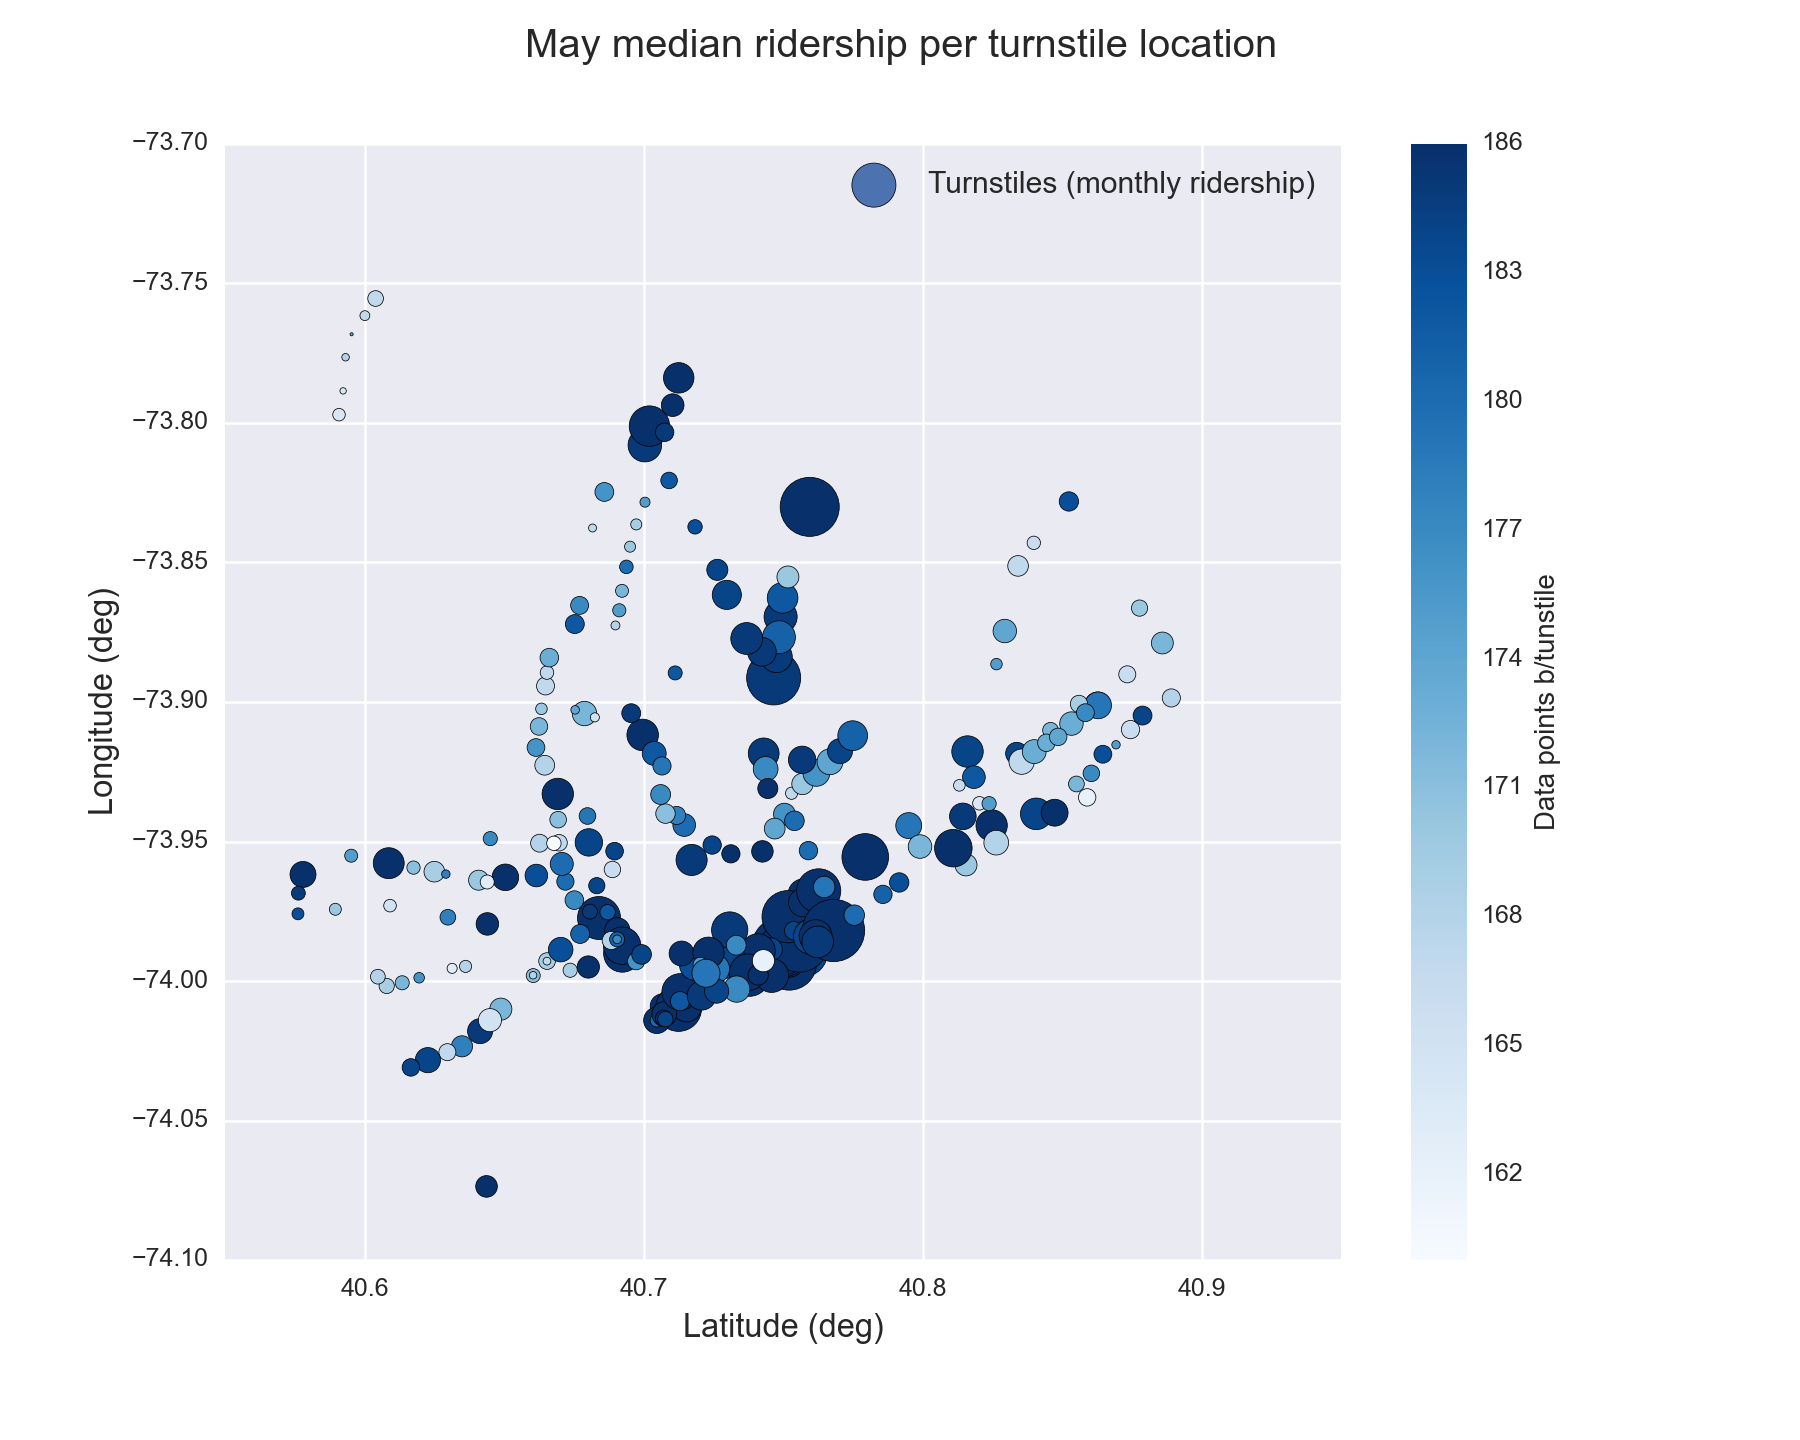
\includegraphics{medrider_loc.png}}
\caption{Turnstiles' locations within NYC, from the improved dataset.}\end{figure}

Besides the information provided by the NYC subway, the dataset also includes
weather information taken from several weather stations within the NYC area:
each turnstile, depending on the location in NYC, is merged with the weather
information of the closest weather station, thus providing temperatures, wind
speed, pressure, conditions, precipitations, etc.

The project focuses one main question: Does the weather conditions, specifically
precipitations, affect the NYC subway ridership? To answer this question we
will use exploratory tools, statistical tests and visualizations. Also, we will
try to fit a model to the data by choosing certain predicting features; will
the use of the precipitation variable improve the fit?


\section{Supporting Material}
\label{overview:supporting-material}
Within the project github repository you will also find an ipython notebook,
where most of the work done was recorded for reference.


\section{Some remarks about the datasets used}
\label{overview:some-remarks-about-the-datasets-used}
For this project we use the data set provided at Data Analyst Nanodegree's
portal for Project 1. The description of the variables can be found on...

However, after the exploratory and data analysis, we created another dataset by
further munging the improved dataset. The basic idea was to smooth out features that
might be caused by individual turnstiles or measurements. To do this, I
grouped the data by time stamp and aggregated the entries by hour by adding all
the entries. Also, the precipitation information for each
time stamp was included by means of two columns:
\begin{itemize}
\item {} 
\code{rain\_hour}: indicator (0 or 1) for precipitations for the particular date
date and time. It is 1 if for any of the stations the conditions were Rain,
Light Rain, Hard Rain or Light Drizzle at that moment.

\item {} 
\code{rain\_day}: indicator (0 or 1) for precipitations for the particular day
of the report. If at any station of our turnstiles the conditions reported
precipitations during the day the value is set to 1.

\end{itemize}


\chapter{Statistical Test}
\label{section1:statistical-test}\label{section1::doc}
In lecture 3 and its problem set, the following question was given \emph{Do rainy}
\emph{days affect the ridership of the NYC subway?} To answer this problem we began by
\begin{quote}

creating two samples from our data:
\end{quote}
\begin{itemize}
\item {} 
Sample A (\emph{No rain}) is a subgroup containing the entries where no rain was reported, using the
information of the \emph{rain} variable (\(rain = 0\))

\item {} 
Sample B (\emph{Rain}) is a subgroup with the entries where some precipitation was reported
by means of the \emph{rain} variable (\(rain = 1\))

\end{itemize}

By studying the distributions, using histograms, we were able to characterize
both data samples. We found out that both samples have a similar shape, clearly
not normal, and positively skewed ({\hyperref[section1:figure21]{\emph{figure 2.1}}}).
\begin{figure}[htbp]
\centering
\capstart

\scalebox{0.600000}{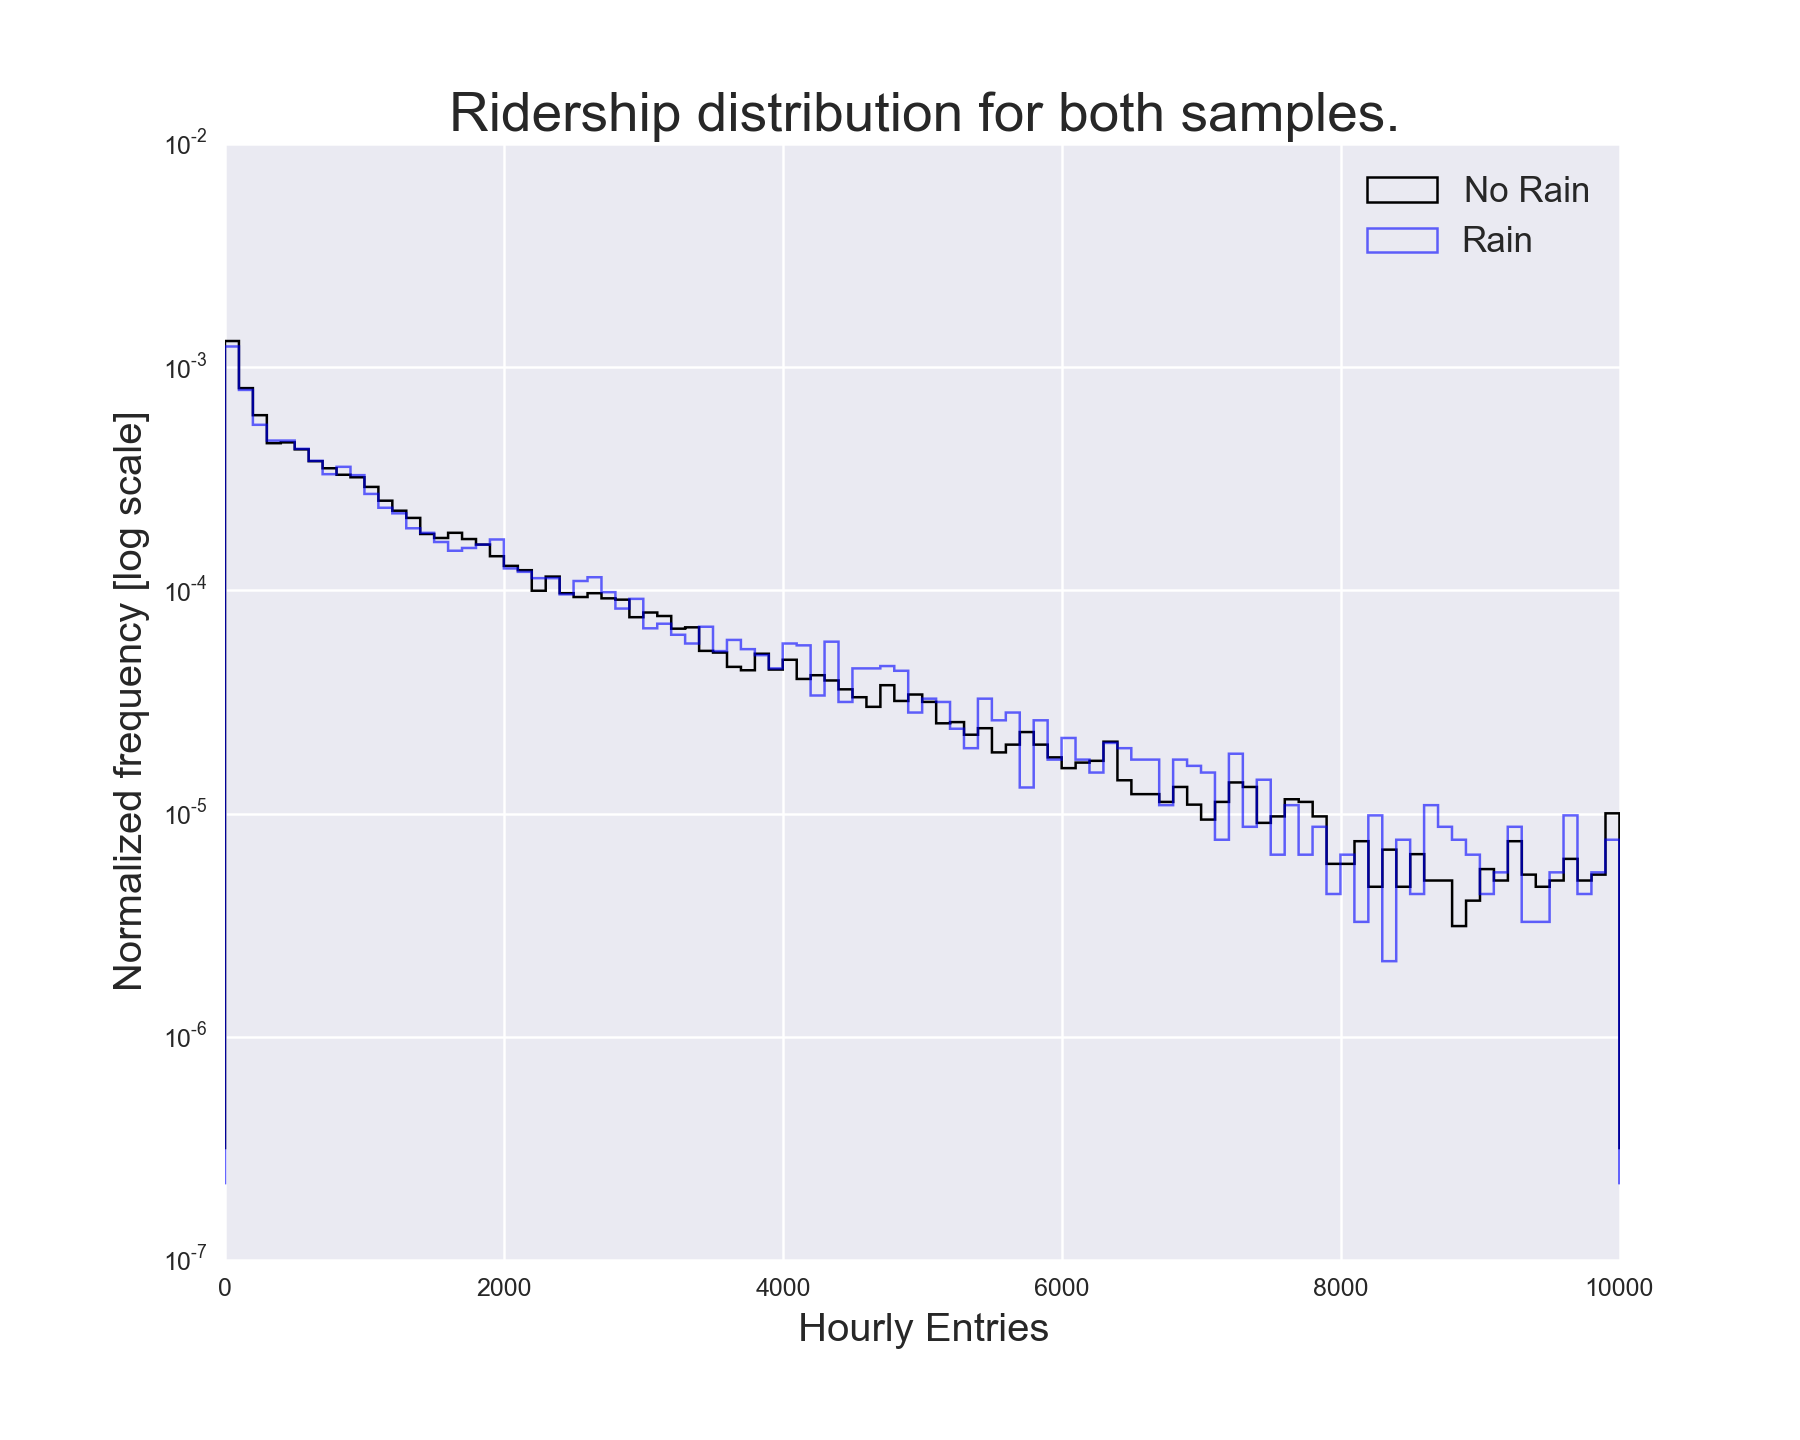
\includegraphics{samples_compared.png}}
\caption{Ridership distribution comparison between rainy and dry days.}{\small 
Please note the logarithmic scale on axis Y. It was used to allows us to study
the visualization with more detail.
}\label{section1:figure21}\end{figure}

Because of the non-normal distribution we decided to use the median as measure
of average for the samples:
\begin{itemize}
\item {} 
Sample A, days without precipitation, show a \textbf{median ridership of}
\textbf{901 passengers per hour.}

\item {} 
Sample B, rainy days, report a \textbf{median of 945 passengers per hour.}

\end{itemize}

To assess the significance of this result, that rain seems to increase ridership
in the NYC system by a small amount, we will use a non-parametric test.


\section{Statistical Test Used}
\label{section1:statistical-test-used}
The Mann Whitney U test is chosen to assess the statistical significance of this
result. The null hypothesis in our case is that both populations are equal, or
that there is no significant deviation on both populations medians (two-tailed
hypothesis).


\section{Justify the Statistical Test}
\label{section1:justify-the-statistical-test}
The Mann Whitney U test, or Wilcoxon rank-sum test, is chosen because of
characteristics of our samples: we can't use a parametric test because the
distributions do not seem to follow any particular and well known probability
distribution which we could use to make inferences that could directly report the
significance of any difference between both populations.

The U test is particularly powerful to assess the significance of the difference
between the median of two samples that have similar distributions. The assumptions
that our data samples must comply with are basically:
\begin{itemize}
\item {} 
All observations of both groups are independent

\item {} 
The responses are ordinal (so we can use the ranking algorithm of the U test).

\end{itemize}


\section{Results}
\label{section1:results}
We used the scipy implementation of the Mann Whitney U test
(scipy.stats.mannwhitneyu). The results from the test are:
\begin{itemize}
\item {} 
\(U = 150678745.0\)

\item {} 
\(p = 1.91 \cdot 10^{-6}\)

\end{itemize}

But the user should be aware that scipy reports p-value for a one-tailed
hypothesis, so we multiply by 2 to get the significance for our hypothesis:
\begin{itemize}
\item {} 
\(p = 3.82 \cdot 10^{-6}\)

\end{itemize}


\section{Interpretation and discussion}
\label{section1:interpretation-and-discussion}
The interpretation, given the result from the U test, is that the the ridership
is not the same for rainy days than non-rainy days, with a significance higher
than 95\% (p \textless{} 0.05). Furthermore, from the descriptive statistics of our samples
we can conclude that the ridership tends to be higher in rainy days.

However we have limited ourselves here to follow the procedure suggested by the
lectures, assuming that observations of both groups are independent and there
no other factors that might wrongly induce this result. Even when the data sample
we use for the project has been through a more complete wrangling, there are
still some issues that might affect the results:
\begin{itemize}
\item {} 
There is missing data for several turnstiles. From the original sample of 240
turnstiles, only 52 have complete data for May; also, as discussed on the forums,
some precipitation data is missing from some weather stations.

\item {} 
We are using the variable \emph{rain} to create our samples: this variable
indicates if the conditions at anytime of the day at a
particular turnstile were rainy. Is it the appropriate variable to use to
build the subgroups?

\item {} 
There is one day which was a holiday (Monday 30th), should the data from this
day be discarded?

\end{itemize}

Let's look with more detail at these problems.


\subsection{Missing data}
\label{section1:missing-data}\begin{figure}[htbp]
\centering
\capstart

\scalebox{0.600000}{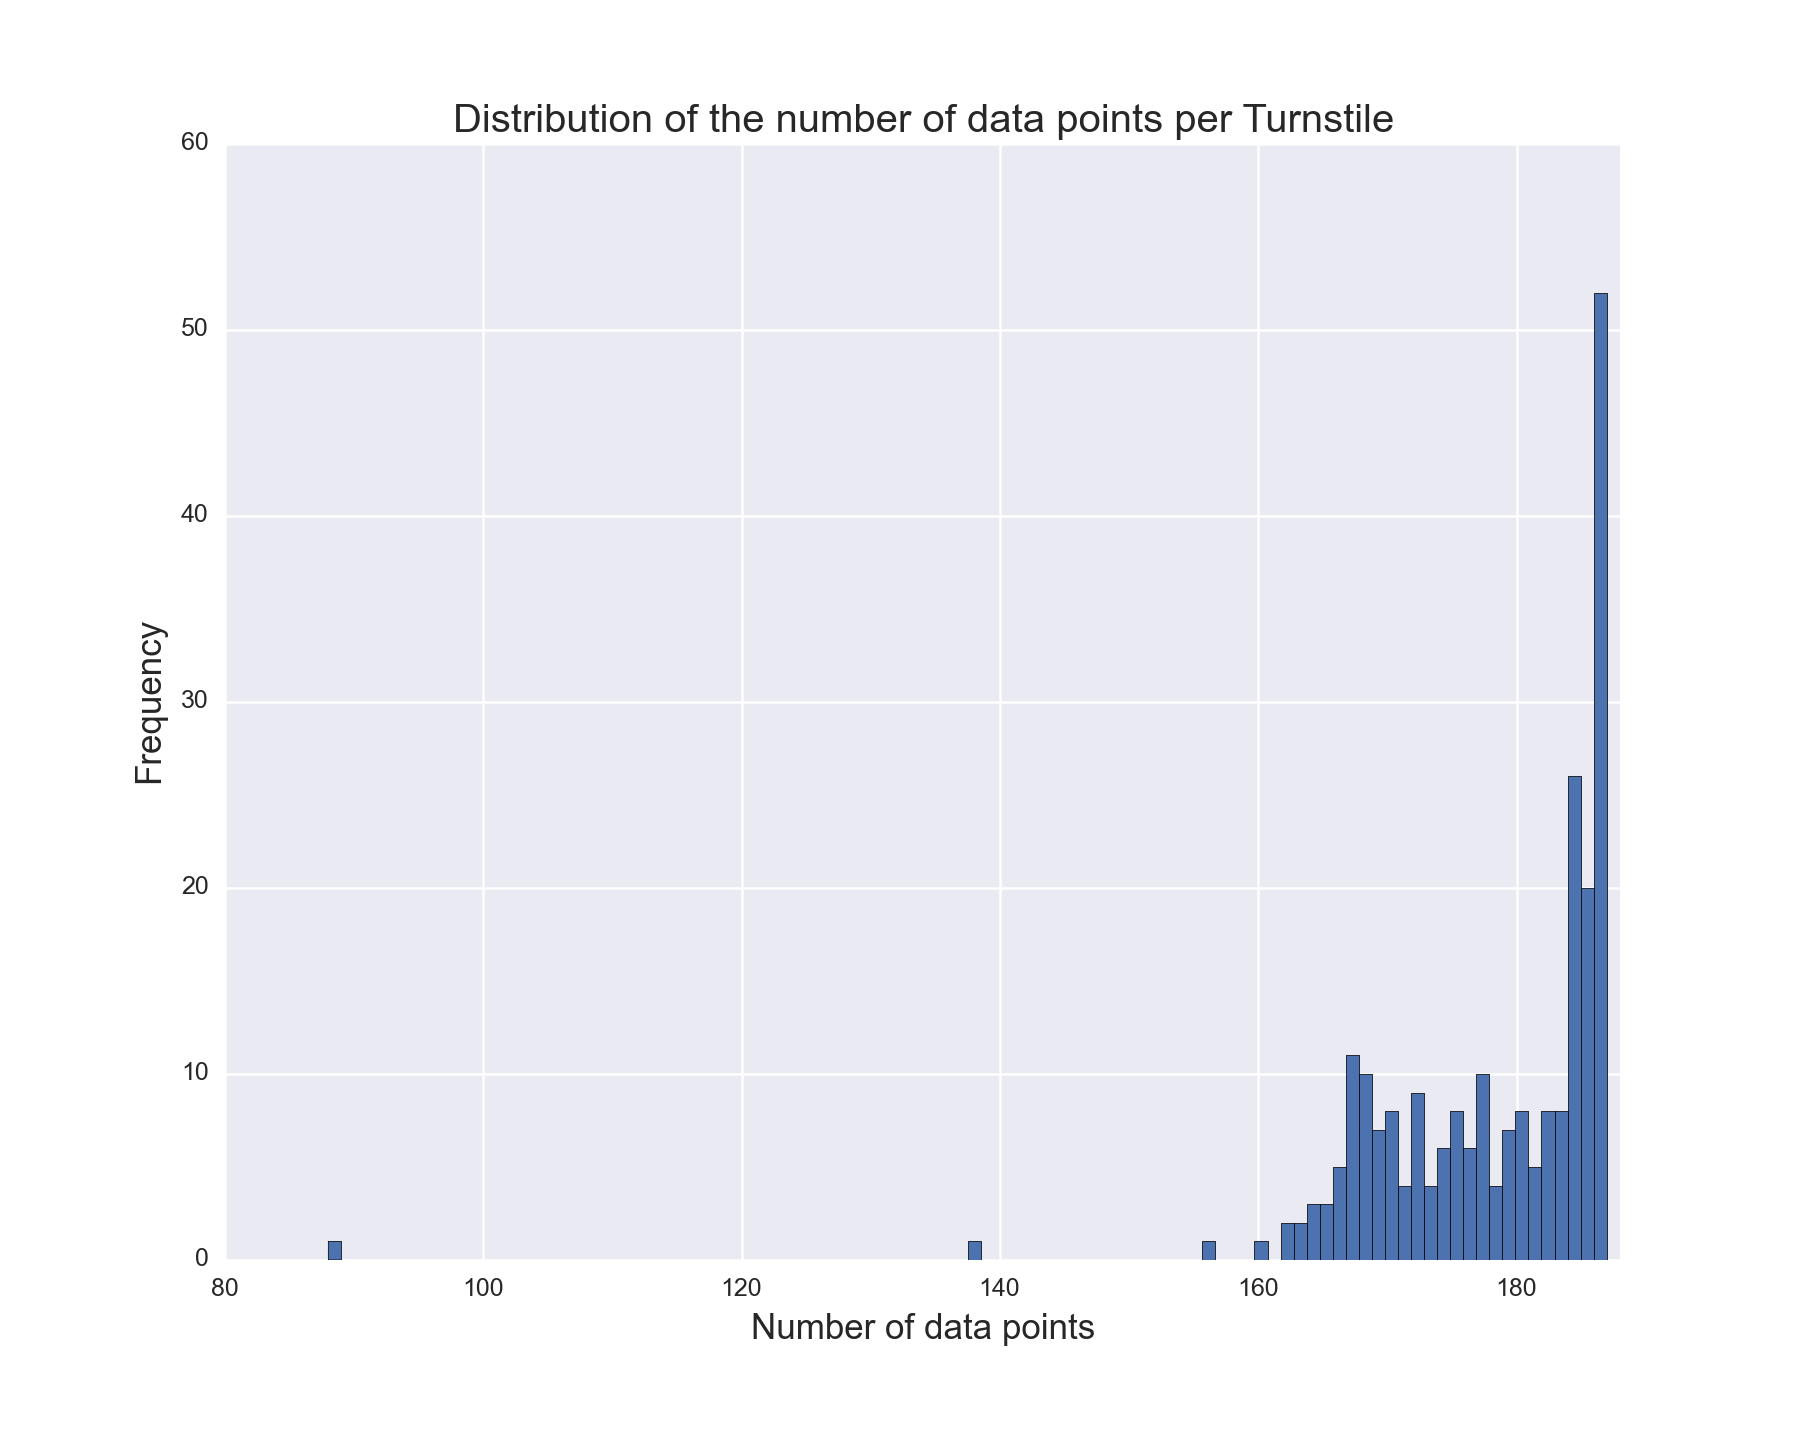
\includegraphics{dataentries.png}}
\caption{Number of data points (measurements) by turnstile on project's improved
dataset.}\label{section1:figure22}\end{figure}

\emph{Figure 2.2} shows some turnstiles have missing data for the
month of May; with 31 days and 6 daily reports it is expected that a complete
monitored turnstile should have 186 measurements. This is the case for 52 turnstiles,
but 185 turnstiles have a number of measurements between 160 and 185. 3 turnstiles
had less than 160 entries, and after inspections they have been removed because
of the huge amount of missing data or time stamps reporting 0 entries. Of the 185
turnstiles with incomplete data, there was one case where at all time stamps the
number of entries was 0, which was also removed as it does not add any information
to our analysis (even when in other cases it could give further information).

The problem with the missing data is that, for some not clear explanation we
could provide, affects more the suburb stations turnstiles than the ones in downtown
areas. And suburb stations tend also to show lower number of hourly entries, i.e, a
lower ridership, than downtown turnstiles. This effect can be seen in
{\hyperref[section1:figure23]{\emph{Figure 2.3}}}.
\begin{figure}[htbp]
\centering
\capstart

\scalebox{0.600000}{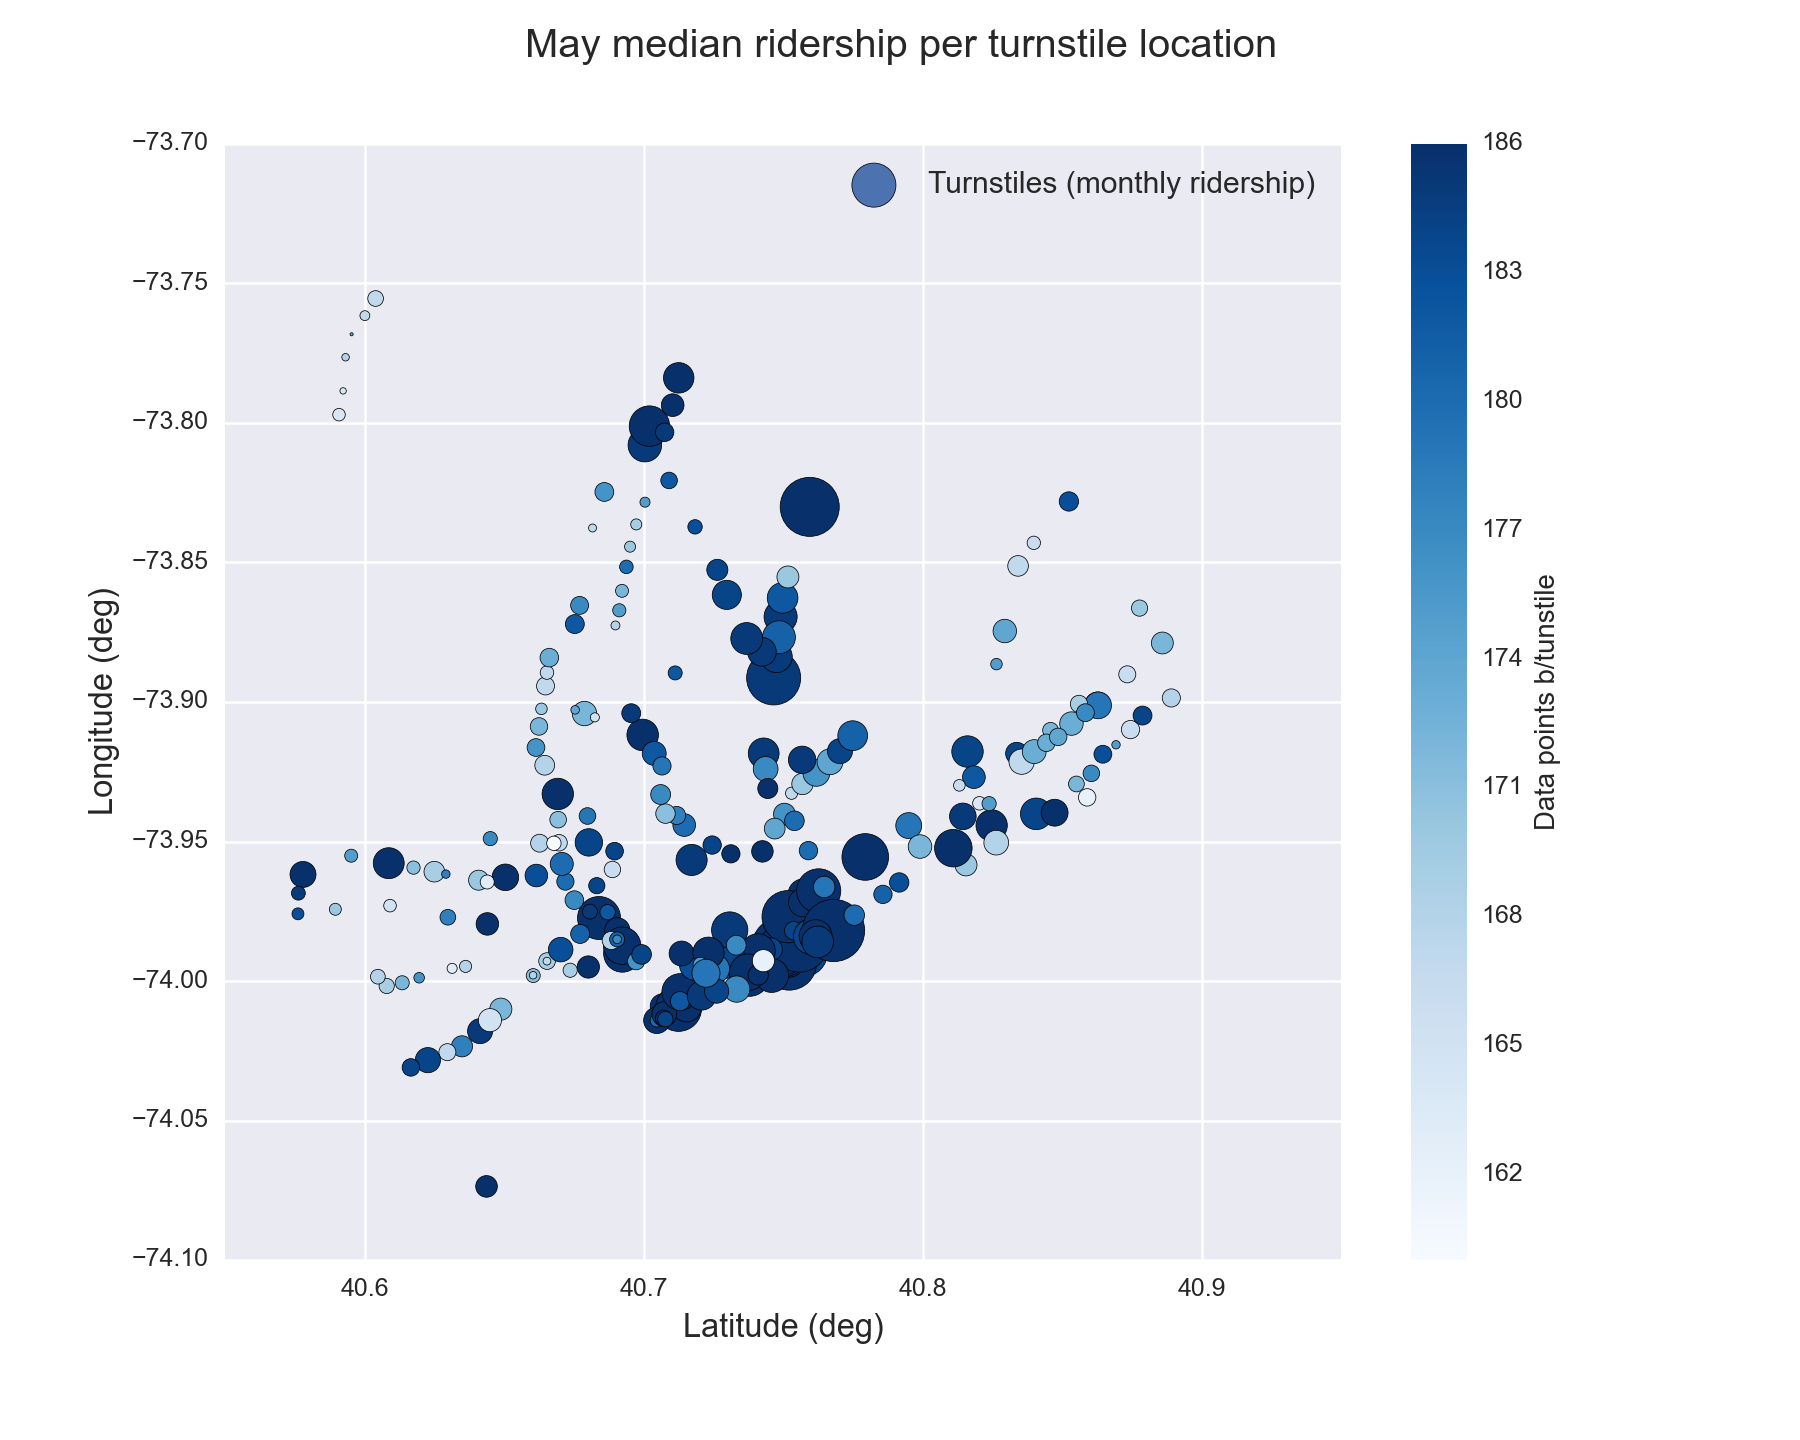
\includegraphics{medrider_loc.png}}
\caption{Turnstiles monthly median ridership, location and number of data points}{\small 
The figure shows the distribution of the turnstiles within NYC which are in
our dataset. The size is proportional to the monthly median ridership (entries
by hour) while the color indicates the data completeness of each turnstile: whiter
colors indicate locations with more missing data.
}\label{section1:figure23}\end{figure}

We, as the reader may, wonder if this missing data could affect in anyway
our previous study. We are not completely sure, but we think that given the way
we performed our analysis it could happen that the results are affected: the downtown
station data, which also correspond to the group of stations with higher ridership,
is contributing to increase the median ``entries by hour'' that we calculate, as they are
located in the higher values side of the ridership distribution. What happens if
the stations in this locations are also the ones that tend to have more rainy days?
We didn't believe this was the case, but just to be sure we created the
plot shown in {\hyperref[section1:figure24]{\emph{Figure 2.4}}}.
\begin{figure}[htbp]
\centering
\capstart

\scalebox{0.600000}{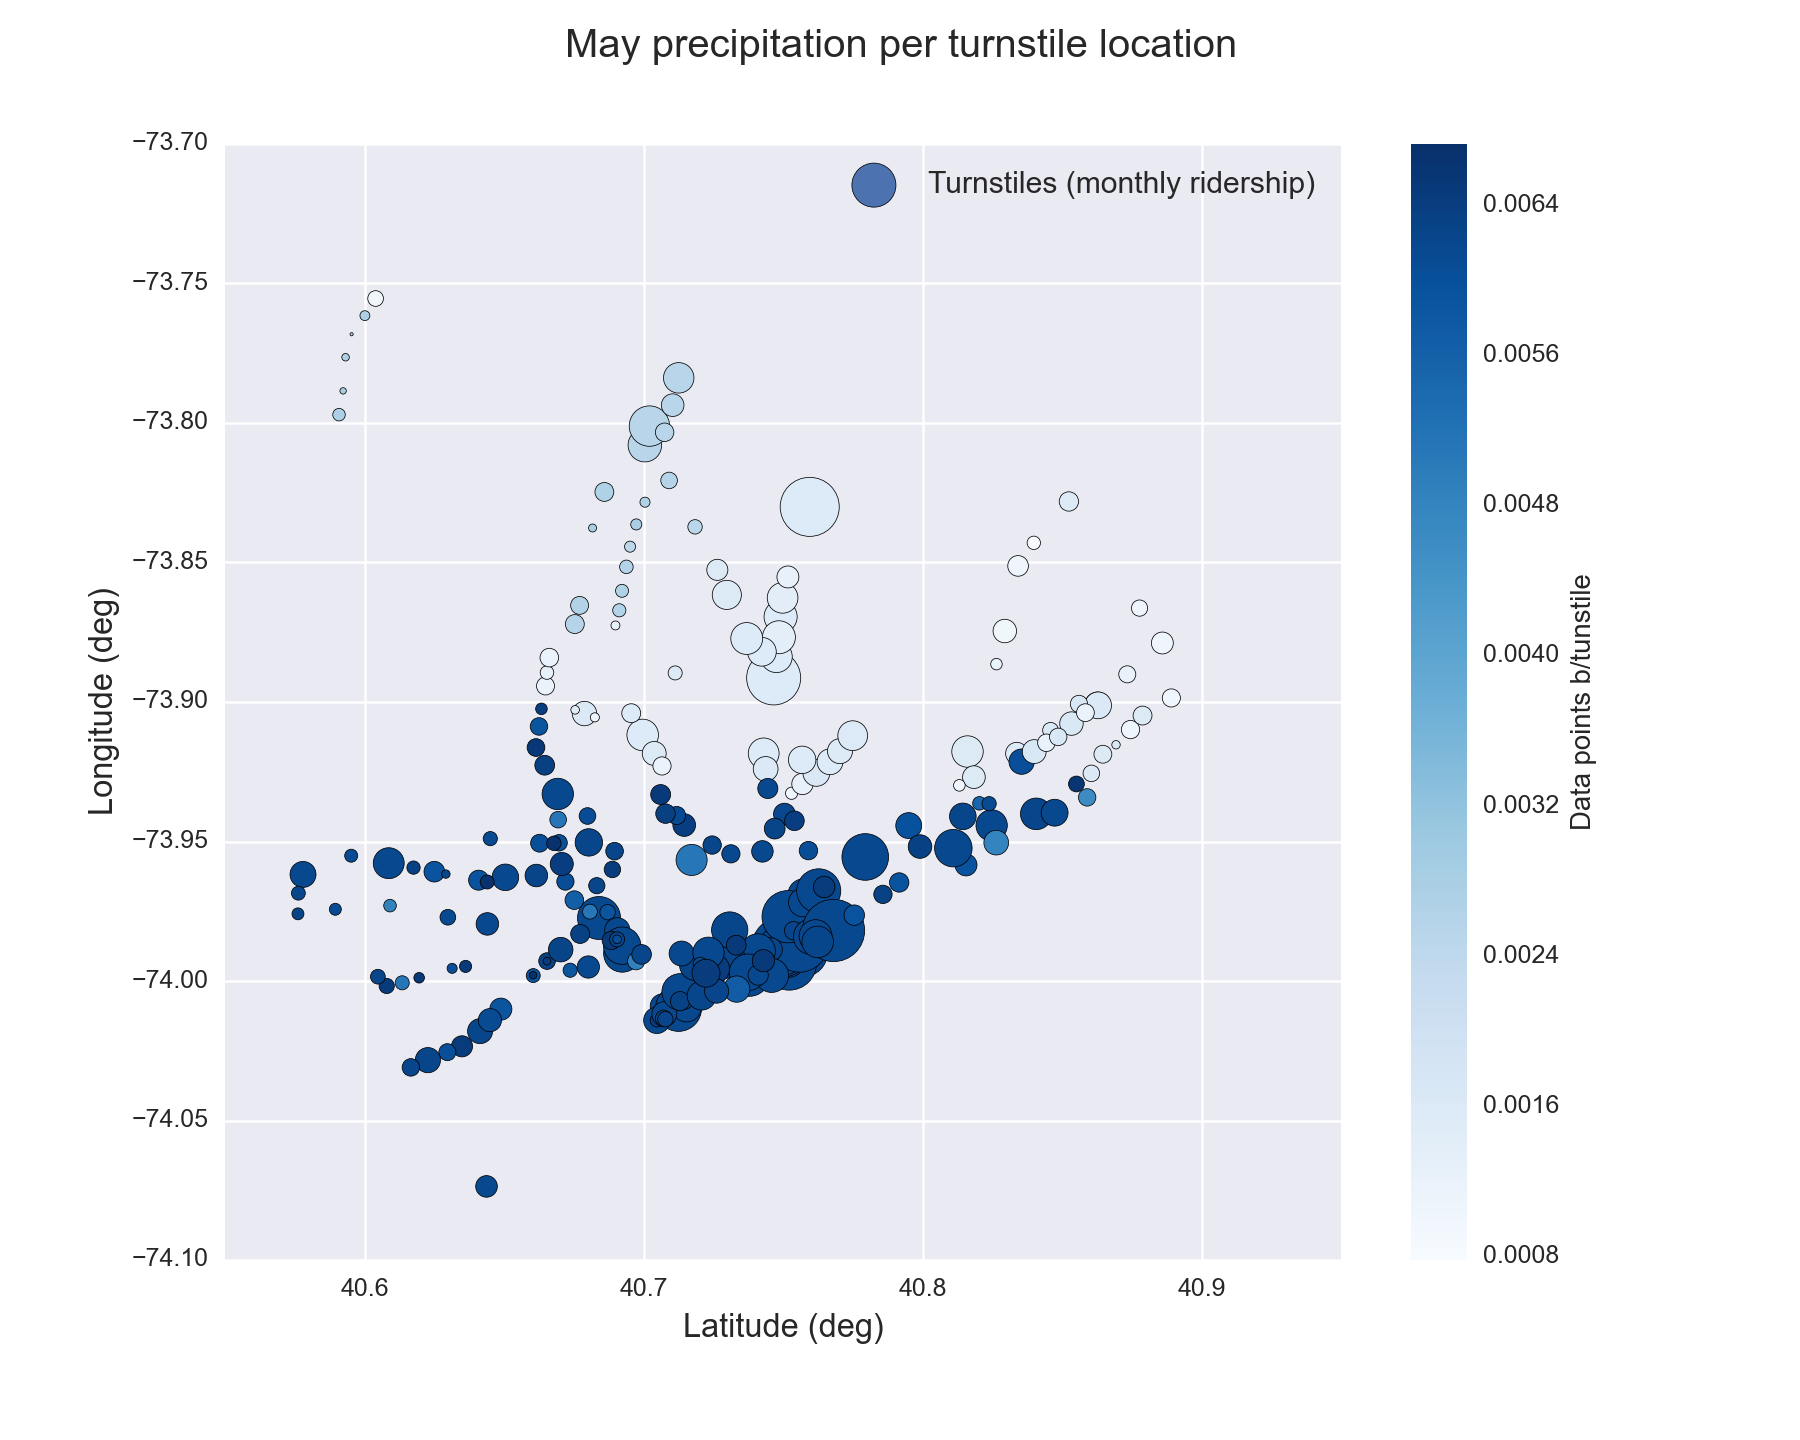
\includegraphics{medprecip_loc.png}}
\caption{Turnstiles monthly median ridership, location and mean precipitation.}{\small 
The figure shows the geographical distribution of the NYC turnstiles in the
project's improved dataset. Size is proportional to the monthly median ridership
and color represent the month's mean precipitation per turnstile. The figure
shows that precipitations are higher in southern (and downtown) NYC.
}\label{section1:figure24}\end{figure}

The figure shows that the precipitation is higher in the northern NYC, which is
also the location of the most busy turnstiles: the median ridership of stations with
higher precipitation (\textgreater{} 0.004 inches) is 1116 entries by hour, while the stations
with lower precipitation (\textless{}= 0.004 inches) is 832 entries by hour. Also the stations
with higher precipitation report on average 7 rainy days while the lower precipitation
turnstiles only report 6.


\chapter{Linear Regression}
\label{section2:linear-regression}\label{section2::doc}

\section{Linear regression algorithm(s)}
\label{section2:linear-regression-algorithm-s}

\subsection{Gradient descent}
\label{section2:gradient-descent}

\subsection{OLS (with statsmodels)}
\label{section2:ols-with-statsmodels}

\section{Features used}
\label{section2:features-used}

\section{Feature selection: why?}
\label{section2:feature-selection-why}

\section{Results: R Squared}
\label{section2:results-r-squared}

\section{Interpretation and limits}
\label{section2:interpretation-and-limits}

\chapter{Visualization}
\label{section3:visualization}\label{section3::doc}

\section{Ridership distribution with weather}
\label{section3:ridership-distribution-with-weather}

\section{Supporting visualizations}
\label{section3:supporting-visualizations}

\chapter{Conclusion}
\label{section4::doc}\label{section4:conclusion}

\chapter{Reflection}
\label{section5::doc}\label{section5:reflection}

\section{Shortcomings and limitations}
\label{section5:shortcomings-and-limitations}

\section{Insights}
\label{section5:insights}


\renewcommand{\indexname}{Index}
\printindex
\end{document}
